\documentclass[twoside]{book}

% Packages required by doxygen
\usepackage{fixltx2e}
\usepackage{calc}
\usepackage{doxygen}
\usepackage{graphicx}
\usepackage[utf8]{inputenc}
\usepackage{makeidx}
\usepackage{multicol}
\usepackage{multirow}
\PassOptionsToPackage{warn}{textcomp}
\usepackage{textcomp}
\usepackage[nointegrals]{wasysym}
\usepackage[table]{xcolor}

% Font selection
\usepackage[T1]{fontenc}
\usepackage{mathptmx}
\usepackage[scaled=.90]{helvet}
\usepackage{courier}
\usepackage{amssymb}
\usepackage{sectsty}
\renewcommand{\familydefault}{\sfdefault}
\allsectionsfont{%
  \fontseries{bc}\selectfont%
  \color{darkgray}%
}
\renewcommand{\DoxyLabelFont}{%
  \fontseries{bc}\selectfont%
  \color{darkgray}%
}
\newcommand{\+}{\discretionary{\mbox{\scriptsize$\hookleftarrow$}}{}{}}

% Page & text layout
\usepackage{geometry}
\geometry{%
  a4paper,%
  top=2.5cm,%
  bottom=2.5cm,%
  left=2.5cm,%
  right=2.5cm%
}
\tolerance=750
\hfuzz=15pt
\hbadness=750
\setlength{\emergencystretch}{15pt}
\setlength{\parindent}{0cm}
\setlength{\parskip}{0.2cm}
\makeatletter
\renewcommand{\paragraph}{%
  \@startsection{paragraph}{4}{0ex}{-1.0ex}{1.0ex}{%
    \normalfont\normalsize\bfseries\SS@parafont%
  }%
}
\renewcommand{\subparagraph}{%
  \@startsection{subparagraph}{5}{0ex}{-1.0ex}{1.0ex}{%
    \normalfont\normalsize\bfseries\SS@subparafont%
  }%
}
\makeatother

% Headers & footers
\usepackage{fancyhdr}
\pagestyle{fancyplain}
\fancyhead[LE]{\fancyplain{}{\bfseries\thepage}}
\fancyhead[CE]{\fancyplain{}{}}
\fancyhead[RE]{\fancyplain{}{\bfseries\leftmark}}
\fancyhead[LO]{\fancyplain{}{\bfseries\rightmark}}
\fancyhead[CO]{\fancyplain{}{}}
\fancyhead[RO]{\fancyplain{}{\bfseries\thepage}}
\fancyfoot[LE]{\fancyplain{}{}}
\fancyfoot[CE]{\fancyplain{}{}}
\fancyfoot[RE]{\fancyplain{}{\bfseries\scriptsize Generated on Mon Sep 1 2014 16\+:17\+:50 for Ad\+Hoc Pathfinder by Doxygen }}
\fancyfoot[LO]{\fancyplain{}{\bfseries\scriptsize Generated on Mon Sep 1 2014 16\+:17\+:50 for Ad\+Hoc Pathfinder by Doxygen }}
\fancyfoot[CO]{\fancyplain{}{}}
\fancyfoot[RO]{\fancyplain{}{}}
\renewcommand{\footrulewidth}{0.4pt}
\renewcommand{\chaptermark}[1]{%
  \markboth{#1}{}%
}
\renewcommand{\sectionmark}[1]{%
  \markright{\thesection\ #1}%
}

% Indices & bibliography
\usepackage{natbib}
\usepackage[titles]{tocloft}
\setcounter{tocdepth}{3}
\setcounter{secnumdepth}{5}
\makeindex

% Hyperlinks (required, but should be loaded last)
\usepackage{ifpdf}
\ifpdf
  \usepackage[pdftex,pagebackref=true]{hyperref}
\else
  \usepackage[ps2pdf,pagebackref=true]{hyperref}
\fi
\hypersetup{%
  colorlinks=true,%
  linkcolor=blue,%
  citecolor=blue,%
  unicode%
}

% Custom commands
\newcommand{\clearemptydoublepage}{%
  \newpage{\pagestyle{empty}\cleardoublepage}%
}


%===== C O N T E N T S =====

\begin{document}

% Titlepage & ToC
\hypersetup{pageanchor=false,
             bookmarks=true,
             bookmarksnumbered=true,
             pdfencoding=unicode
            }
\pagenumbering{roman}
\begin{titlepage}
\vspace*{7cm}
\begin{center}%
{\Large Ad\+Hoc Pathfinder }\\
\vspace*{1cm}
{\large Generated by Doxygen 1.8.8}\\
\vspace*{0.5cm}
{\small Mon Sep 1 2014 16:17:50}\\
\end{center}
\end{titlepage}
\clearemptydoublepage
\tableofcontents
\clearemptydoublepage
\pagenumbering{arabic}
\hypersetup{pageanchor=true}

%--- Begin generated contents ---
\chapter{Hierarchical Index}
\section{Class Hierarchy}
This inheritance list is sorted roughly, but not completely, alphabetically\+:\begin{DoxyCompactList}
\item \contentsline{section}{A\+Star\+Ad\+Hoc\+Pathfinder\+Node}{\pageref{class_a_star_ad_hoc_pathfinder_node}}{}
\item \contentsline{section}{Binary\+Heap}{\pageref{class_binary_heap}}{}
\item Mono\+Behaviour\begin{DoxyCompactList}
\item \contentsline{section}{A\+Star\+Ad\+Hoc\+Pathfinder}{\pageref{class_a_star_ad_hoc_pathfinder}}{}
\item \contentsline{section}{A\+Star\+Ad\+Hoc\+Simple\+Movement}{\pageref{class_a_star_ad_hoc_simple_movement}}{}
\end{DoxyCompactList}
\end{DoxyCompactList}

\chapter{Class Index}
\section{Class List}
Here are the classes, structs, unions and interfaces with brief descriptions\+:\begin{DoxyCompactList}
\item\contentsline{section}{\hyperlink{class_a_star_ad_hoc_pathfinder}{A\+Star\+Ad\+Hoc\+Pathfinder} }{\pageref{class_a_star_ad_hoc_pathfinder}}{}
\item\contentsline{section}{\hyperlink{class_a_star_ad_hoc_pathfinder_node}{A\+Star\+Ad\+Hoc\+Pathfinder\+Node} }{\pageref{class_a_star_ad_hoc_pathfinder_node}}{}
\item\contentsline{section}{\hyperlink{class_a_star_ad_hoc_simple_movement}{A\+Star\+Ad\+Hoc\+Simple\+Movement} }{\pageref{class_a_star_ad_hoc_simple_movement}}{}
\item\contentsline{section}{\hyperlink{class_binary_heap}{Binary\+Heap} }{\pageref{class_binary_heap}}{}
\end{DoxyCompactList}

\chapter{Class Documentation}
\hypertarget{class_a_star_ad_hoc_pathfinder}{\section{A\+Star\+Ad\+Hoc\+Pathfinder Class Reference}
\label{class_a_star_ad_hoc_pathfinder}\index{A\+Star\+Ad\+Hoc\+Pathfinder@{A\+Star\+Ad\+Hoc\+Pathfinder}}
}
Inheritance diagram for A\+Star\+Ad\+Hoc\+Pathfinder\+:\begin{figure}[H]
\begin{center}
\leavevmode
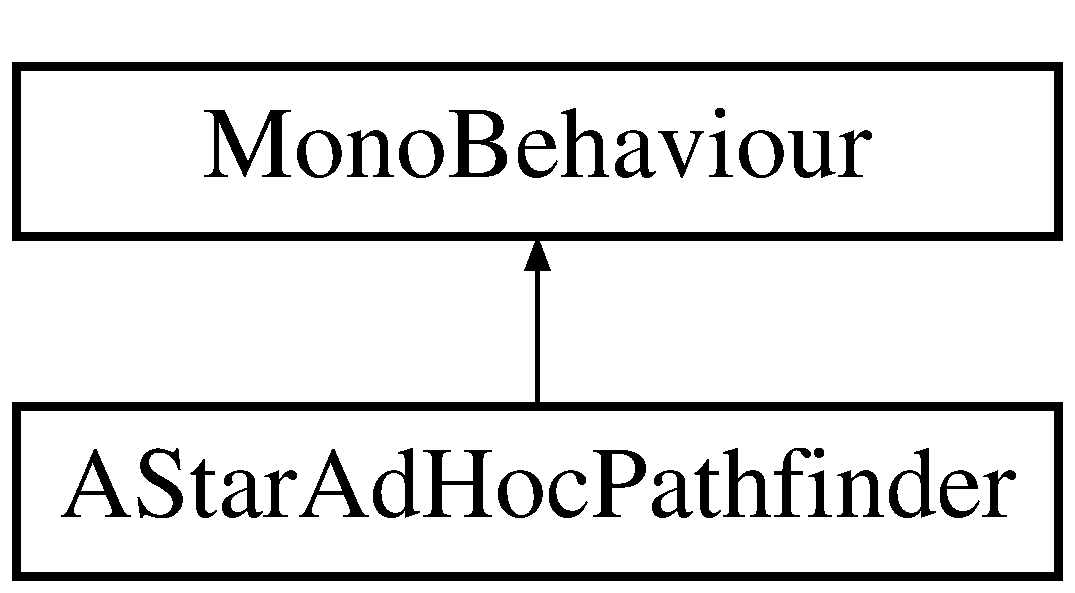
\includegraphics[height=2.000000cm]{class_a_star_ad_hoc_pathfinder}
\end{center}
\end{figure}
\subsection*{Public Member Functions}
\begin{DoxyCompactItemize}
\item 
\hypertarget{class_a_star_ad_hoc_pathfinder_aa31719400e49672181dd2becf4b6c259}{void {\bfseries Reset} ()}\label{class_a_star_ad_hoc_pathfinder_aa31719400e49672181dd2becf4b6c259}

\item 
\hypertarget{class_a_star_ad_hoc_pathfinder_a2029b90076e70929f9ed3f524359235c}{void {\bfseries Find\+Path\+To\+Target} ()}\label{class_a_star_ad_hoc_pathfinder_a2029b90076e70929f9ed3f524359235c}

\item 
\hypertarget{class_a_star_ad_hoc_pathfinder_a2855db3735ca99c2f7e8038c6594aacc}{I\+Enumerator {\bfseries Find\+Path\+To\+Target\+Corutine} ()}\label{class_a_star_ad_hoc_pathfinder_a2855db3735ca99c2f7e8038c6594aacc}

\item 
\hypertarget{class_a_star_ad_hoc_pathfinder_a9d9516c7f212bf9cfe828ae2f0250210}{Array\+List {\bfseries Post\+Process\+Node\+List} (\hyperlink{class_a_star_ad_hoc_pathfinder_node}{A\+Star\+Ad\+Hoc\+Pathfinder\+Node} last\+Node)}\label{class_a_star_ad_hoc_pathfinder_a9d9516c7f212bf9cfe828ae2f0250210}

\item 
\hypertarget{class_a_star_ad_hoc_pathfinder_a87b5cf69f5cd3ce7509c1522e933cb5c}{Array\+List {\bfseries Smooth\+Path} (Array\+List original\+List, int passes=1)}\label{class_a_star_ad_hoc_pathfinder_a87b5cf69f5cd3ce7509c1522e933cb5c}

\end{DoxyCompactItemize}
\subsection*{Public Attributes}
\begin{DoxyCompactItemize}
\item 
\hypertarget{class_a_star_ad_hoc_pathfinder_a82f51112de52a07caaf5c3b41d2627e0}{Game\+Object {\bfseries start\+Object}}\label{class_a_star_ad_hoc_pathfinder_a82f51112de52a07caaf5c3b41d2627e0}

\item 
\hypertarget{class_a_star_ad_hoc_pathfinder_a7a63e627a73d1c2af28890ddb8af27b6}{Game\+Object {\bfseries target\+Object}}\label{class_a_star_ad_hoc_pathfinder_a7a63e627a73d1c2af28890ddb8af27b6}

\item 
\hypertarget{class_a_star_ad_hoc_pathfinder_a394691b3ce1650ff721f5bf699fff716}{Vector3 {\bfseries start}}\label{class_a_star_ad_hoc_pathfinder_a394691b3ce1650ff721f5bf699fff716}

\item 
\hypertarget{class_a_star_ad_hoc_pathfinder_aaf05f59ce751f7ef833a83f47612b715}{Vector3 {\bfseries target}}\label{class_a_star_ad_hoc_pathfinder_aaf05f59ce751f7ef833a83f47612b715}

\item 
\hypertarget{class_a_star_ad_hoc_pathfinder_ab28b625bb5905f006d2e0beb7fe57d24}{float {\bfseries nav\+Resolution} = 1.\+0f}\label{class_a_star_ad_hoc_pathfinder_ab28b625bb5905f006d2e0beb7fe57d24}

\item 
\hypertarget{class_a_star_ad_hoc_pathfinder_a1afdba50b759e4e40b831b7c07d4c428}{float {\bfseries max\+Angle} = 45.\+0f}\label{class_a_star_ad_hoc_pathfinder_a1afdba50b759e4e40b831b7c07d4c428}

\item 
\hypertarget{class_a_star_ad_hoc_pathfinder_a981722b4cf02ca028a6b4cedef516225}{string\mbox{[}$\,$\mbox{]} {\bfseries out\+Of\+Bounds\+Tags}}\label{class_a_star_ad_hoc_pathfinder_a981722b4cf02ca028a6b4cedef516225}

\item 
\hypertarget{class_a_star_ad_hoc_pathfinder_a83ea32f20565d3f7343f9c01a329d90f}{float {\bfseries search\+Timeout} = 10.\+0f}\label{class_a_star_ad_hoc_pathfinder_a83ea32f20565d3f7343f9c01a329d90f}

\item 
\hypertarget{class_a_star_ad_hoc_pathfinder_acc0e58382409ccdce59cd1f0dff9a098}{bool {\bfseries use\+Optimal\+Heuristics} = false}\label{class_a_star_ad_hoc_pathfinder_acc0e58382409ccdce59cd1f0dff9a098}

\item 
\hypertarget{class_a_star_ad_hoc_pathfinder_a942bfa694d184dc2dd5a8cfbabc9e1e2}{int {\bfseries raycast\+Height} = 1000}\label{class_a_star_ad_hoc_pathfinder_a942bfa694d184dc2dd5a8cfbabc9e1e2}

\item 
\hypertarget{class_a_star_ad_hoc_pathfinder_ac0f41f95ca333743a366a10b971c0b95}{bool {\bfseries finished\+Pathfinding} = false}\label{class_a_star_ad_hoc_pathfinder_ac0f41f95ca333743a366a10b971c0b95}

\item 
\hypertarget{class_a_star_ad_hoc_pathfinder_a90ff1223c39ad8cab56e12a2b9af2d53}{\hyperlink{class_a_star_ad_hoc_pathfinder_node}{A\+Star\+Ad\+Hoc\+Pathfinder\+Node} {\bfseries first\+Node} = null}\label{class_a_star_ad_hoc_pathfinder_a90ff1223c39ad8cab56e12a2b9af2d53}

\item 
\hypertarget{class_a_star_ad_hoc_pathfinder_acce294950bb47098968b8810d5ab6458}{int {\bfseries cycles\+Per\+Frame} = 2}\label{class_a_star_ad_hoc_pathfinder_acce294950bb47098968b8810d5ab6458}

\item 
\hypertarget{class_a_star_ad_hoc_pathfinder_a295cf9cb0c092444d21af48574117f25}{bool {\bfseries debug\+Mode} = false}\label{class_a_star_ad_hoc_pathfinder_a295cf9cb0c092444d21af48574117f25}

\item 
\hypertarget{class_a_star_ad_hoc_pathfinder_a43bf5a9dc164a0f6efae2561ebf58faf}{Game\+Object {\bfseries debug\+Open\+List\+Object} = null}\label{class_a_star_ad_hoc_pathfinder_a43bf5a9dc164a0f6efae2561ebf58faf}

\item 
\hypertarget{class_a_star_ad_hoc_pathfinder_a27db7ab0f99553e9bb4c4c52e381a5a8}{Game\+Object {\bfseries debug\+Closed\+List\+Object} = null}\label{class_a_star_ad_hoc_pathfinder_a27db7ab0f99553e9bb4c4c52e381a5a8}

\item 
\hypertarget{class_a_star_ad_hoc_pathfinder_a51528372e4ef74eeadda1fb0a63acdf4}{Game\+Object {\bfseries debug\+Path\+Object} = null}\label{class_a_star_ad_hoc_pathfinder_a51528372e4ef74eeadda1fb0a63acdf4}

\item 
\hypertarget{class_a_star_ad_hoc_pathfinder_a0ad514d62484d2a5df20f640809ddfbd}{G\+U\+I\+Text {\bfseries debug\+Text\+Status}}\label{class_a_star_ad_hoc_pathfinder_a0ad514d62484d2a5df20f640809ddfbd}

\end{DoxyCompactItemize}


The documentation for this class was generated from the following file\+:\begin{DoxyCompactItemize}
\item 
Z\+:/\+Github\+\_\+repos/\+Ad\+Hoc-\/\+Pathfinder/code/A\+Star\+Ad\+Hoc\+Pathfinder.\+cs\end{DoxyCompactItemize}

\hypertarget{class_a_star_ad_hoc_pathfinder_node}{\section{A\+Star\+Ad\+Hoc\+Pathfinder\+Node Class Reference}
\label{class_a_star_ad_hoc_pathfinder_node}\index{A\+Star\+Ad\+Hoc\+Pathfinder\+Node@{A\+Star\+Ad\+Hoc\+Pathfinder\+Node}}
}
\subsection*{Public Member Functions}
\begin{DoxyCompactItemize}
\item 
\hypertarget{class_a_star_ad_hoc_pathfinder_node_a2718609f883d9975f8b4fbd9f95a6412}{void {\bfseries Update\+Weight} ()}\label{class_a_star_ad_hoc_pathfinder_node_a2718609f883d9975f8b4fbd9f95a6412}

\end{DoxyCompactItemize}
\subsection*{Public Attributes}
\begin{DoxyCompactItemize}
\item 
\hypertarget{class_a_star_ad_hoc_pathfinder_node_a6c2f4394cbf3eb9ea30fb72d4c6a4ebb}{float {\bfseries origin\+Cost}}\label{class_a_star_ad_hoc_pathfinder_node_a6c2f4394cbf3eb9ea30fb72d4c6a4ebb}

\item 
\hypertarget{class_a_star_ad_hoc_pathfinder_node_a5a2bec42c2855c8cbc3e6df3224dd775}{float {\bfseries destin\+Cost}}\label{class_a_star_ad_hoc_pathfinder_node_a5a2bec42c2855c8cbc3e6df3224dd775}

\item 
\hypertarget{class_a_star_ad_hoc_pathfinder_node_ae1b9e6c89f4b1a9d2a12b5a5e520fc80}{float {\bfseries weight}}\label{class_a_star_ad_hoc_pathfinder_node_ae1b9e6c89f4b1a9d2a12b5a5e520fc80}

\item 
\hypertarget{class_a_star_ad_hoc_pathfinder_node_a4a628a1213b57baff66fbdfe5ddfa888}{\hyperlink{class_a_star_ad_hoc_pathfinder_node}{A\+Star\+Ad\+Hoc\+Pathfinder\+Node} {\bfseries parent}}\label{class_a_star_ad_hoc_pathfinder_node_a4a628a1213b57baff66fbdfe5ddfa888}

\item 
\hypertarget{class_a_star_ad_hoc_pathfinder_node_a09cfa2bf7fe21191830e9fe1369c6479}{Vector3 {\bfseries position}}\label{class_a_star_ad_hoc_pathfinder_node_a09cfa2bf7fe21191830e9fe1369c6479}

\item 
\hypertarget{class_a_star_ad_hoc_pathfinder_node_ad0ce5befc74dcd258bb915974da520f8}{string {\bfseries hash\+Code}}\label{class_a_star_ad_hoc_pathfinder_node_ad0ce5befc74dcd258bb915974da520f8}

\end{DoxyCompactItemize}


The documentation for this class was generated from the following file\+:\begin{DoxyCompactItemize}
\item 
Z\+:/\+Github\+\_\+repos/\+Ad\+Hoc-\/\+Pathfinder/code/A\+Star\+Ad\+Hoc\+Pathfinder.\+cs\end{DoxyCompactItemize}

\hypertarget{class_a_star_ad_hoc_simple_movement}{\section{A\+Star\+Ad\+Hoc\+Simple\+Movement Class Reference}
\label{class_a_star_ad_hoc_simple_movement}\index{A\+Star\+Ad\+Hoc\+Simple\+Movement@{A\+Star\+Ad\+Hoc\+Simple\+Movement}}
}
Inheritance diagram for A\+Star\+Ad\+Hoc\+Simple\+Movement\+:\begin{figure}[H]
\begin{center}
\leavevmode
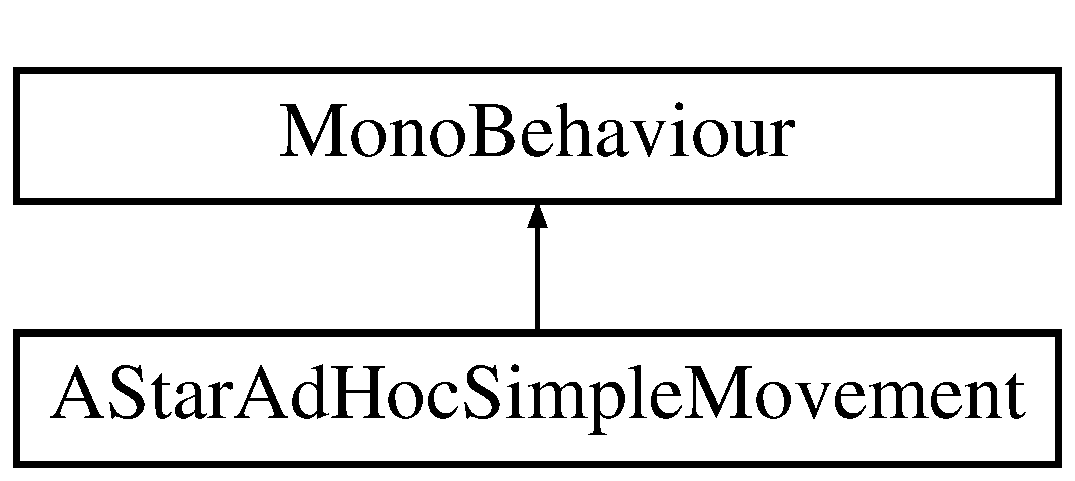
\includegraphics[height=2.000000cm]{class_a_star_ad_hoc_simple_movement}
\end{center}
\end{figure}
\subsection*{Public Member Functions}
\begin{DoxyCompactItemize}
\item 
\hypertarget{class_a_star_ad_hoc_simple_movement_acc2668195bbf5a95507928e5db30d416}{void {\bfseries Set\+New\+Target\+Position} (Vector3 target\+Position, bool auto\+Start\+Movement=false)}\label{class_a_star_ad_hoc_simple_movement_acc2668195bbf5a95507928e5db30d416}

\item 
\hypertarget{class_a_star_ad_hoc_simple_movement_a0335a43825fae28dae0d7cbdfa2fac63}{void {\bfseries Pause\+Movement} ()}\label{class_a_star_ad_hoc_simple_movement_a0335a43825fae28dae0d7cbdfa2fac63}

\item 
\hypertarget{class_a_star_ad_hoc_simple_movement_acdcac131bf797fe5e4964e47905529bc}{void {\bfseries Continue\+Movement} ()}\label{class_a_star_ad_hoc_simple_movement_acdcac131bf797fe5e4964e47905529bc}

\end{DoxyCompactItemize}
\subsection*{Public Attributes}
\begin{DoxyCompactItemize}
\item 
\hypertarget{class_a_star_ad_hoc_simple_movement_a5f9b53189df1d5b040206d2ce967cd59}{float {\bfseries speed} = 1.\+0f}\label{class_a_star_ad_hoc_simple_movement_a5f9b53189df1d5b040206d2ce967cd59}

\item 
\hypertarget{class_a_star_ad_hoc_simple_movement_a11913c5cc0e4a1e4ecf76c1270475202}{bool {\bfseries is\+Moving} = false}\label{class_a_star_ad_hoc_simple_movement_a11913c5cc0e4a1e4ecf76c1270475202}

\item 
\hypertarget{class_a_star_ad_hoc_simple_movement_a0f2745c874b2589caa4dab61e05f0b16}{bool {\bfseries debug\+Mode} = false}\label{class_a_star_ad_hoc_simple_movement_a0f2745c874b2589caa4dab61e05f0b16}

\item 
\hypertarget{class_a_star_ad_hoc_simple_movement_a783f7c2da13202c27f1f2b458e767765}{Game\+Object {\bfseries target\+G\+O}}\label{class_a_star_ad_hoc_simple_movement_a783f7c2da13202c27f1f2b458e767765}

\end{DoxyCompactItemize}


The documentation for this class was generated from the following file\+:\begin{DoxyCompactItemize}
\item 
Z\+:/\+Github\+\_\+repos/\+Ad\+Hoc-\/\+Pathfinder/code/A\+Star\+Ad\+Hoc\+Simple\+Movement.\+cs\end{DoxyCompactItemize}

\hypertarget{class_binary_heap}{\section{Binary\+Heap Class Reference}
\label{class_binary_heap}\index{Binary\+Heap@{Binary\+Heap}}
}
\subsection*{Public Member Functions}
\begin{DoxyCompactItemize}
\item 
\hypertarget{class_binary_heap_ad1d6cdbc7082a7ec2dddb3bac6035c0c}{void {\bfseries Add} (\hyperlink{class_a_star_ad_hoc_pathfinder_node}{A\+Star\+Ad\+Hoc\+Pathfinder\+Node} node)}\label{class_binary_heap_ad1d6cdbc7082a7ec2dddb3bac6035c0c}

\item 
\hypertarget{class_binary_heap_a50f1f939f056e0cc738d42375f39ec76}{\hyperlink{class_a_star_ad_hoc_pathfinder_node}{A\+Star\+Ad\+Hoc\+Pathfinder\+Node} {\bfseries Remove} ()}\label{class_binary_heap_a50f1f939f056e0cc738d42375f39ec76}

\item 
\hypertarget{class_binary_heap_a497314219c8a3480c4367181e205acf6}{void {\bfseries Update} (\hyperlink{class_a_star_ad_hoc_pathfinder_node}{A\+Star\+Ad\+Hoc\+Pathfinder\+Node} node)}\label{class_binary_heap_a497314219c8a3480c4367181e205acf6}

\item 
\hypertarget{class_binary_heap_a0c99f3665cc24018023293dfbd20f147}{int {\bfseries Index\+Of\+Node\+With\+Hash\+Code} (string node\+Hash\+Code)}\label{class_binary_heap_a0c99f3665cc24018023293dfbd20f147}

\item 
\hypertarget{class_binary_heap_a4902196f0ec8753aedc0e73f9d8c4de4}{\hyperlink{class_a_star_ad_hoc_pathfinder_node}{A\+Star\+Ad\+Hoc\+Pathfinder\+Node} {\bfseries Node\+With\+Hash\+Code} (string node\+Hash\+Code)}\label{class_binary_heap_a4902196f0ec8753aedc0e73f9d8c4de4}

\item 
\hypertarget{class_binary_heap_abc5643e14a9ef074c1234bb2be369e88}{int {\bfseries Count} ()}\label{class_binary_heap_abc5643e14a9ef074c1234bb2be369e88}

\item 
\hypertarget{class_binary_heap_ae7f594ee113018ca8ded3947906bf0c3}{virtual I\+Dictionary\+Enumerator {\bfseries Get\+Enumerator} ()}\label{class_binary_heap_ae7f594ee113018ca8ded3947906bf0c3}

\end{DoxyCompactItemize}


The documentation for this class was generated from the following file\+:\begin{DoxyCompactItemize}
\item 
Z\+:/\+Github\+\_\+repos/\+Ad\+Hoc-\/\+Pathfinder/code/A\+Star\+Ad\+Hoc\+Pathfinder.\+cs\end{DoxyCompactItemize}

%--- End generated contents ---

% Index
\newpage
\phantomsection
\addcontentsline{toc}{chapter}{Index}
\printindex

\end{document}
